
\documentclass[letterpaper,hide notes,xcolor={table,svgnames},pdftex,10pt]{beamer}
\def\showexamples{t}


%\usepackage[svgnames]{xcolor}

%% Demo talk
%\documentclass[letterpaper,notes=show]{beamer}

\usecolortheme{crane}
\setbeamertemplate{navigation symbols}{}

\usetheme{MyPittsburgh}
%\usetheme{Frankfurt}

%\usepackage{tipa}

\usepackage{hyperref}
\usepackage{graphicx,xspace}
\usepackage[normalem]{ulem}
\usepackage{multicol}
\usepackage{amsmath,amssymb,amsthm,graphicx,xspace}
\newcommand\SF[1]{$\bigstar$\footnote{SF: #1}}

\usepackage[default]{sourcesanspro}
\usepackage[T1]{fontenc}

\newcounter{tmpnumSlide}
\newcounter{tmpnumNote}

% old question code
%\newcommand\question[1]{{$\bigstar$ \small \onlySlide{2}{#1}}}
% \newcommand\nquestion[1]{\ifdefined \presentationonly \textcircled{?} \fi \note{\par{\Large \textbf{?}} #1}}
% \newcommand\nanswer[1]{\note{\par{\Large \textbf{A}} #1}}


 \newcommand\mnote[1]{%
   \addtocounter{tmpnumSlide}{1}
   \ifdefined\showcues {~\tiny\fbox{\arabic{tmpnumSlide}}}\fi
   \note{\setlength{\parskip}{1ex}\addtocounter{tmpnumNote}{1}\textbf{\Large \arabic{tmpnumNote}:} {#1\par}}}

\newcommand\mmnote[1]{\note{\setlength{\parskip}{1ex}#1\par}}

%\newcommand\mnote[2][]{\ifdefined\handoutwithnotes {~\tiny\fbox{#1}}\fi
% \note{\setlength{\parskip}{1ex}\textbf{\Large #1:} #2\par}}

%\newcommand\mnote[2][]{{\tiny\fbox{#1}} \note{\setlength{\parskip}{1ex}\textbf{\Large #1:} #2\par}}

\newcommand\mquestion[2]{{~\color{red}\fbox{?}}\note{\setlength{\parskip}{1ex}\par{\Large \textbf{?}} #1} \note{\setlength{\parskip}{1ex}\par{\Large \textbf{A}} #2\par}\ifdefined \presentationonly \pause \fi}

\newcommand\blackboard[1]{%
\ifdefined   \showblackboard
  {#1}
  \else {\begin{center} \fbox{\colorbox{blue!30}{%
         \begin{minipage}{.95\linewidth}%
           \hspace{\stretch{1}} Some space intentionally left blank; done at the blackboard.%
         \end{minipage}}}\end{center}}%
         \fi%
}



%\newcommand\q{\tikz \node[thick,color=black,shape=circle]{?};}
%\newcommand\q{\ifdefined \presentationonly \textcircled{?} \fi}

\usepackage{listings}
\lstset{%
  keywordstyle=\bfseries,
  aboveskip=15pt,
  belowskip=15pt,
  captionpos=b,
  identifierstyle=\ttfamily,
  escapeinside={(*@}{@*)},
  stringstyle=\ttfamiliy,
  frame=lines,
  numbers=left, basicstyle=\scriptsize, numberstyle=\tiny, stepnumber=0, numbersep=2pt}

\usepackage{siunitx}
\newcommand\sius[1]{\num[group-separator = {,}]{#1}\si{\micro\second}}
\newcommand\sims[1]{\num[group-separator = {,}]{#1}\si{\milli\second}}
\newcommand\sins[1]{\num[group-separator = {,}]{#1}\si{\nano\second}}
\sisetup{group-separator = {,}, group-digits = true}

%% -------------------- tikz --------------------
\usepackage{tikz}
\usetikzlibrary{positioning}
\usetikzlibrary{arrows,backgrounds,automata,decorations.shapes,decorations.pathmorphing,decorations.markings,decorations.text}

\tikzstyle{place}=[circle,draw=blue!50,fill=blue!20,thick, inner sep=0pt,minimum size=6mm]
\tikzstyle{transition}=[rectangle,draw=black!50,fill=black!20,thick, inner sep=0pt,minimum size=4mm]

\tikzstyle{block}=[rectangle,draw=black, thick, inner sep=5pt]
\tikzstyle{bullet}=[circle,draw=black, fill=black, thin, inner sep=2pt]

\tikzstyle{pre}=[<-,shorten <=1pt,>=stealth',semithick]
\tikzstyle{post}=[->,shorten >=1pt,>=stealth',semithick]
\tikzstyle{bi}=[<->,shorten >=1pt,shorten <=1pt, >=stealth',semithick]

\tikzstyle{mut}=[-,>=stealth',semithick]

\tikzstyle{treereset}=[dashed,->, shorten >=1pt,>=stealth',thin]

\usepackage{ifmtarg}
\usepackage{xifthen}
\makeatletter
% new counter to now which frame it is within the sequence
\newcounter{multiframecounter}
% initialize buffer for previously used frame title
\gdef\lastframetitle{\textit{undefined}}
% new environment for a multi-frame
\newenvironment{multiframe}[1][]{%
\ifthenelse{\isempty{#1}}{%
% if no frame title was set via optional parameter,
% only increase sequence counter by 1
\addtocounter{multiframecounter}{1}%
}{%
% new frame title has been provided, thus
% reset sequence counter to 1 and buffer frame title for later use
\setcounter{multiframecounter}{1}%
\gdef\lastframetitle{#1}%
}%
% start conventional frame environment and
% automatically set frame title followed by sequence counter
\begin{frame}%
\frametitle{\lastframetitle~{\normalfont(\arabic{multiframecounter})}}%
}{%
\end{frame}%
}
\makeatother

\makeatletter
\newdimen\tu@tmpa%
\newdimen\ydiffl%
\newdimen\xdiffl%
\newcommand\ydiff[2]{%
    \coordinate (tmpnamea) at (#1);%
    \coordinate (tmpnameb) at (#2);%
    \pgfextracty{\tu@tmpa}{\pgfpointanchor{tmpnamea}{center}}%
    \pgfextracty{\ydiffl}{\pgfpointanchor{tmpnameb}{center}}%
    \advance\ydiffl by -\tu@tmpa%
}
\newcommand\xdiff[2]{%
    \coordinate (tmpnamea) at (#1);%
    \coordinate (tmpnameb) at (#2);%
    \pgfextractx{\tu@tmpa}{\pgfpointanchor{tmpnamea}{center}}%
    \pgfextractx{\xdiffl}{\pgfpointanchor{tmpnameb}{center}}%
    \advance\xdiffl by -\tu@tmpa%
}
\makeatother
\newcommand{\copyrightbox}[3][r]{%
\begin{tikzpicture}%
\node[inner sep=0pt,minimum size=2em](ciimage){#2};
\usefont{OT1}{phv}{n}{n}\fontsize{4}{4}\selectfont
\ydiff{ciimage.south}{ciimage.north}
\xdiff{ciimage.west}{ciimage.east}
\ifthenelse{\equal{#1}{r}}{%
\node[inner sep=0pt,right=1ex of ciimage.south east,anchor=north west,rotate=90]%
{\raggedleft\color{black!50}\parbox{\the\ydiffl}{\raggedright{}#3}};%
}{%
\ifthenelse{\equal{#1}{l}}{%
\node[inner sep=0pt,right=1ex of ciimage.south west,anchor=south west,rotate=90]%
{\raggedleft\color{black!50}\parbox{\the\ydiffl}{\raggedright{}#3}};%
}{%
\node[inner sep=0pt,below=1ex of ciimage.south west,anchor=north west]%
{\raggedleft\color{black!50}\parbox{\the\xdiffl}{\raggedright{}#3}};%
}
}
\end{tikzpicture}
}


%% --------------------

%\usepackage[excludeor]{everyhook}
%\PushPreHook{par}{\setbox0=\lastbox\llap{MUH}}\box0}

%\vspace*{\stretch{1}

%\setbox0=\lastbox \llap{\textbullet\enskip}\box0}

\setlength{\parskip}{\fill}

\newcommand\noskips{\setlength{\parskip}{1ex}}
\newcommand\doskips{\setlength{\parskip}{\fill}}

\newcommand\xx{\par\vspace*{\stretch{1}}\par}
\newcommand\xxs{\par\vspace*{2ex}\par}
\newcommand\tuple[1]{\langle #1 \rangle}
\newcommand\code[1]{{\sf \footnotesize #1}}
\newcommand\ex[1]{\uline{Example:} \ifdefined \presentationonly \pause \fi
  \ifdefined\showexamples#1\xspace\else{\uline{\hspace*{2cm}}}\fi}

\newcommand\ceil[1]{\lceil #1 \rceil}


\AtBeginSection[]
{
   \begin{frame}
       \frametitle{Outline}
       \tableofcontents[currentsection]
   \end{frame}
}



\pgfdeclarelayer{edgelayer}
\pgfdeclarelayer{nodelayer}
\pgfsetlayers{edgelayer,nodelayer,main}

\tikzstyle{none}=[inner sep=0pt]
\tikzstyle{rn}=[circle,fill=Red,draw=Black,line width=0.8 pt]
\tikzstyle{gn}=[circle,fill=Lime,draw=Black,line width=0.8 pt]
\tikzstyle{yn}=[circle,fill=Yellow,draw=Black,line width=0.8 pt]
\tikzstyle{empty}=[circle,fill=White,draw=Black]
\tikzstyle{bw} = [rectangle, draw, fill=blue!20, 
    text width=4em, text centered, rounded corners, minimum height=2em]
    
    \newcommand{\CcNote}[1]{% longname
	This work is licensed under the \textit{Creative Commons #1 3.0 License}.%
}
\newcommand{\CcImageBy}[1]{%
	\includegraphics[scale=#1]{creative_commons/cc_by_30.pdf}%
}
\newcommand{\CcImageSa}[1]{%
	\includegraphics[scale=#1]{creative_commons/cc_sa_30.pdf}%
}
\newcommand{\CcImageNc}[1]{%
	\includegraphics[scale=#1]{creative_commons/cc_nc_30.pdf}%
}
\newcommand{\CcGroupBySa}[2]{% zoom, gap
	\CcImageBy{#1}\hspace*{#2}\CcImageNc{#1}\hspace*{#2}\CcImageSa{#1}%
}
\newcommand{\CcLongnameByNcSa}{Attribution-NonCommercial-ShareAlike}

\newenvironment{changemargin}[1]{% 
  \begin{list}{}{% 
    \setlength{\topsep}{0pt}% 
    \setlength{\leftmargin}{#1}% 
    \setlength{\rightmargin}{1em}
    \setlength{\listparindent}{\parindent}% 
    \setlength{\itemindent}{\parindent}% 
    \setlength{\parsep}{\parskip}% 
  }% 
  \item[]}{\end{list}} 




\def\ojoin{\setbox0=\hbox{$\bowtie$}%
  \rule[-.02ex]{.25em}{.4pt}\llap{\rule[\ht0]{.25em}{.4pt}}}
\def\leftouterjoin{\mathbin{\ojoin\mkern-5.8mu\bowtie}}

\title{Tutorial 10 --- Parallelism and Distributed Databases }

\author{Richard Wong \\ \small \texttt{rk2wong@edu.uwaterloo.ca}}
\institute{Department of Electrical and Computer Engineering \\
  University of Waterloo}
\date{\today}


\begin{document}

\begin{frame}
  \titlepage

\end{frame}

\begin{frame}
\frametitle{Contacting Me}

If you have a question that you are okay with sharing publicly prior to the final exam, visit \texttt{https://github.com/rwongone/ece356/issues} and open a new issue.

You can still email me at \texttt{rk2wong@edu.uwaterloo.ca}, but for the benefit of your peers I may ask for your permission to share your question and my answer via the Issues page.

\end{frame}

\begin{frame}
\frametitle{Exercise 10-1}

What kinds of queries are the following partitioning schemes well-suited for?

\begin{enumerate}
  \item round-robin
  \item range partitioning
  \item hash partitioning
\end{enumerate}

\end{frame}


\begin{frame}
\frametitle{Exercise 10-1 Solution}

\begin{enumerate}
  \item round-robin: good for high-selectivity queries; tuples of a single relation are spread out evenly throughout the $n$ disks, so load is also balanced. not as good for point queries and range queries, since we can't know ahead of time which disk the tuples reside on.
  \item range partitioning: good for point and range queries on the partitioning attribute, since we can quickly find out the disk or range of disks that the tuples reside on.
  \item hash partitioning: good for point queries on the partitioning attribute. Also good for high-selectivity queries since tuples are evenly distributed.
\end{enumerate}

\end{frame}


\begin{frame}
\frametitle{Exercise 10-2}

How would a distributed DB using the following partitioning schemes handle \textbf{addition} of nodes?

\begin{enumerate}
  \item round-robin
  \item range partitioning
  \item hash partitioning
\end{enumerate}

\end{frame}



\begin{frame}
\frametitle{Exercise 10-2 Solution (1/2)}

\begin{enumerate}
  \item round-robin: need to recompute which partition each tuple will go to. Recall the partition is decided by some counter mod $n$, but by adding a new node, $n$ changes.
  \item range partitioning: the new node is responsible for a new range, and takes data from the nodes responsible for the ranges on its left and right.
  \item hash partitioning: if we implement this naively, (i.e. partition is $h(x)$ mod $n$), then do the same as in round robin; not great.
\end{enumerate}

\end{frame}


\begin{frame}
\frametitle{Exercise 10-2 Solution (2/2)}

Note: we can use a "distributed hash table" to make node addition with hash partitioning more like it is with range partitioning. One implementation is called Chord.

tldr: "Hash the tuples, but also hash the nodes. Each node is responsible for the range of hashes to its right."

\begin{center}
  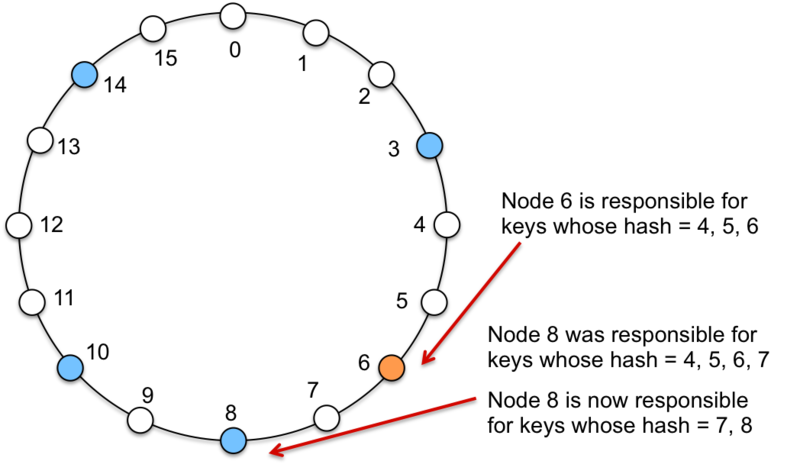
\includegraphics[width=0.75\textwidth]{images/dht-chord-new_node.png}\\
\end{center}

Credit for image: https://www.cs.rutgers.edu/~pxk/417/notes/23-lookup.html

\end{frame}


\begin{frame}
\frametitle{Exercise 10-3}

Distinguish between the following:

\begin{enumerate}
  \item attribute-value skew
  \item partition skew
  \item execution skew
\end{enumerate}

\end{frame}


\begin{frame}
\frametitle{Exercise 10-3 Solution}

\begin{enumerate}
  \item attribute-value skew: many tuples with the same attribute or packed in a tight range of attributes reside on a single partition.
  \item partition skew: partitions carry uneven quantities of tuples, independently of attribute-value skew. This seems to be an effect of random chance, or a poor partitioning scheme.
  \item execution skew: during the execution of a query, a few disks may contain most of the tuples to access, while other have very few or none. This creates an I/O bottleneck, and is also known as \textit{load imbalance}.
\end{enumerate}

\end{frame}


\begin{frame}
\frametitle{Exercise 10-4}

What factors would account for \textbf{execution skew} in the following partitioning schemes?

\begin{enumerate}
  \item range partitioning
  \item hash partitioning
\end{enumerate}

\end{frame}


\begin{frame}
\frametitle{Exercise 10-4 Solution}

Attribute-value skew tends to lead to execution skew, in both range- and hash- partitioning.

A naive implementation of range partitioning will allocate most of the load to a small number of disks (just the ones that cover the query range).

\end{frame}


\begin{frame}
\frametitle{Exercise 10-5}

How can we alleviate the problem of load imbalance in range partitioning?

\end{frame}


\begin{frame}
\frametitle{Exercise 10-5 Solution}

One strategy is to use \textbf{virtual processors}.

Pretend that there are many more virtual processors as there are real processors.

Instead of mapping real processors to attribute ranges, we map the many virtual processors to attribute ranges, then balance the virtual processors among the real processors.

This causes our ranges to be split more finely, and also distributed evenly among the disks, causing range queries to hit a greater number of disks, which allows for greater parallelism.

\end{frame}


\begin{frame}
\frametitle{Exercise 10-6}

Suppose we have the following relation: \\
\begin{center}
  \texttt{employee(name, address, salary, plantNumber)}
\end{center}

The relation is \textbf{fragmented horizontally} by \texttt{plantNumber}, \\
and each fragment has a \textbf{local replica}, \\
and a \textbf{replica in New York}.

Provide a reasonable processing strategy for each of the following queries \textbf{made from the plant in Montreal}:

\begin{enumerate}
  \item Find all employees at the Toronto plant.
  \item Find the average salary of all employees.
  \item Find the highest-paid employee in Toronto, Vancouver, and Edmonton.
\end{enumerate}

\end{frame}


\begin{frame}
\frametitle{Exercise 10-6 Solution}

\begin{center}
  \texttt{employee(name, address, salary, plantNumber)}
\end{center}

\begin{enumerate}
  \item Find all employees at the Toronto plant:
    \begin{enumerate}
      \item send the query to Toronto
      \item process in Toronto
      \item receive the result from Toronto
    \end{enumerate}
  \item Find the average salary of all employees:
    \begin{enumerate}
      \item send the query to New York
      \item compute the average in New York, since it has a replica of all fragments
      \item receive the result from New York
    \end{enumerate}
  \item Find the highest-paid employee in Toronto, Vancouver, and Edmonton:
    \begin{enumerate}
      \item send query to Toronto, Vancouver, and Edmonton
      \item compute max at those sites to take advantage of parallelism
      \item receive results Toronto, Vancouver, and Edmonton
      \item aggregate in Montreal
    \end{enumerate}
\end{enumerate}

\end{frame}

\end{document}
